\begin{dang}{Sự tương giao của hai đồ thị}
	\begin{enumerate}[\iconCH]
		\item \indamm{Xác định tọa độ giao điểm của hai đồ thị $y=f(x)$ và $y=g(x)$:}
		\begin{listEX}[1]
			\item [\ding{172}] Giải phương trình hoành độ giao điểm $f(x)=g(x)$, tìm các nghiệm $x_0 \in \mathscr{D}_f \cap \mathscr{D}_g$.
			\item [\ding{173}] Với $x_0$ vừa tìm, thay vào một trong hai hàm số ban đầu để tìm $y_0$.
			\item [\ding{174}] Kết luận giao điểm $(x_0;y_0)$.
		\end{listEX}
		\item \indamm{Ứng dụng đồ thị để biện luận nghiệm phương trình:}
		\immini{
		\begin{enumerate}[]
			\item Xét phương trình $f(x)=m$, với $m$ là tham số. Nghiệm của phương trình này có thể coi là hoành độ giao điểm của đồ thị $y=f(x)$ (cố định) với đường thẳng $y=m$ (nằm ngang).
			\item Từ đó, để biện luận nghiệm phương trình $f(x)=m$, ta có thể thực hiện các bước như sau:
				\begin{itemize}
					\item [$\bullet$] Lập bảng biến thiên của hàm số $y=f(x)$ trên miền xác định mà đề bài yêu cầu.
					\item [$\bullet$] Tịnh tiến đường thẳng $y=m$ theo hướng "\textit{lên, xuống}". Quan sát số giao điểm để quy ra số nghiệm tương ứng.
				\end{itemize}
		\end{enumerate}}{
	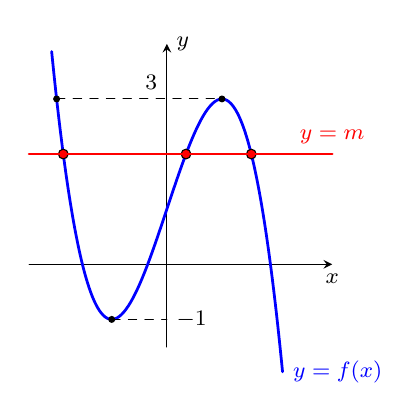
\begin{tikzpicture}[scale=0.7, font=\footnotesize, line join=round, line cap=round, >=stealth]
		\draw[->] (-2.5,0) -- (3,0) node[below]{ $x$};
		\draw[->] (0,-1.5) -- (0,4) node[right]{ $y$};
		\draw[blue,line width=1pt,smooth,samples=100,domain=-2.09:2.1] plot(\x,{-(\x)^3+3*(\x)+1})node[right]{\footnotesize $y=f(x)$};
		\draw[dashed](-2,3)--(0,3)node[above left]{\footnotesize $3$}--(1,3);
		\draw[dashed](-1,-1)--(0,-1)node[right]{\footnotesize $-1$};
		\draw[fill=black] (-2,3) circle(1.5pt) (-1,-1) circle(1.5pt) (1,3) circle(1.5pt);
		\draw[fill=red] (0.3473,2) circle(2.5pt) (1.5321,2) circle(2.5pt) (-1.8794,2) circle(2.5pt);
		\draw[line width=1pt,red](-2.5,2)--(3,2)node[above]{\footnotesize $y=m$};
\end{tikzpicture}}
	\end{enumerate}
\end{dang}
\boxmini{BÀI TẬP TỰ LUẬN}
\begin{vd}
	Xác định tọa độ giao điểm của hai đồ thị hàm số sau:
	\begin{tasks}(2)
		\task $y=x^3-2x^2+x-1$ và $y=1-2x$;
		\task $y=\dfrac{x+8}{x-2}$ và $y=x+2$.
	\end{tasks}
\loigiai{
\begin{enumerate}[a)]
	\item Xét phương trình hoành độ giao điểm\\
	\centerline{$x^3-2x^2+x-1=1-2x\Leftrightarrow x^3-2x^2+3x-2=0\Leftrightarrow(x-1)\left(x^2-x+2\right)=0\Leftrightarrow x=1$.}\\
	Do đó $2$ đồ thị  hàm số có giao điểm là $(1;-1)$.
	\item Với điều kiện $x\ne 2$ ta có\\
	Phương trình hoành độ giao điểm $x+2=\dfrac{x+8}{x-2}\Leftrightarrow x^2-4=x+8 \Leftrightarrow x^2 -x -12 =0 \Leftrightarrow \hoac{&x=3\\&x=-4.}$\\
	Từ đó được $A(3;5)$ và $B(-4;-2)$.
\end{enumerate}}
\end{vd}

\begin{vd}
	Tìm tập hợp các giá trị thực của tham số $m$  để đồ thị hàm số $y=(x-2)(x^2+mx+m^2-3)$ cắt trục hoành tại ba điểm phân biệt.
	\loigiai{
		Đồ thị hàm số đã cho cắt trục hoành tại ba điểm phân biệt khi phương trình $$(x-2)(x^2+mx+m^2-3)=0$$ có $3$ nghiệm phân biệt hay phương trình $x^2+mx+m^2-3=0$ có $2$ nghiệm phân biệt khác $2$ 
		$$\Leftrightarrow \heva{\Delta& =-3m^2+12>0\\m&^2+2m+1\ne 0}\Leftrightarrow \heva{-&2<m<2\\m&\ne -1}.$$
	}
\end{vd}

\begin{vd}
	Tìm tham số m để phương trình $x^3 - 3x + 2-m=0$ có ba nghiệm phân biệt.
	\loigiai{
		Phương trình tương đương với  $x^3 - 3x + 2=m$.
		\immini {
			\begin{itemize}
				\item [$\bullet$] Số nghiệm của phương trình bằng số giao điểm của đồ thị $y=x^3 - 3x + 2$ với đường thẳng $y=m$ (nằm ngang).
				\item [$\bullet$] Đồ thị hàm số $ y = x^3 - 3x +2 $ như hình bên. Để đường thẳng $ y = m $ cắt đồ thị tại 3 điểm phân biệt khi và chỉ khi $ 0 < m < 4. $
			\end{itemize}
		Vậy $ 0 < m < 4. $
			}
		{\begin{tikzpicture}[>=stealth,scale=0.6,every node/.style={scale=0.8}]
				\draw[->,black] (-2.5,0) -- (3,0)node[above left] {$x$};
				từ tọa độ (-1.5,0) đến tạo độ (3.5,0) ghi tên x ở trên bên trái
				\draw[->,black] (0,-1) -- (0,4.5)node[right] {$y$};
				\foreach \x in {-1,1,2}
				\draw[shift={(\x,0)}] (0pt,1pt) -- (0pt,-1pt) node[below] {\footnotesize $\x$};
				\foreach \y in {2,3,4}
				\draw[shift={(0,\y)}] (1pt,0pt) -- (-1pt,0pt) node[right] {\footnotesize $\y$};
				\node at (0,0) [below right] {\footnotesize $O$};
				\draw[smooth,samples=100,domain=-2.1:2.02] plot(\x,{(\x)^3-3*(\x)+2});
				\draw [dashed] (-1,0)--(-1,4)--(0,4);
				\draw [blue] (-2.4,2.5)--(2.9,2.5);
				\node at (2,2.5) [below right] {\footnotesize $y=m$};
			\end{tikzpicture}
		}
	}
\end{vd}

\boxmini{BÀI TẬP TRẮC NGHIỆM}
\setcounter{ex}{0}
\Opensolutionfile{ans}[ans/2D1-B4-d4-1]
\begin{ex}%[2D1B5-4]
	Đường thẳng $y=x-1$ cắt đồ thị hàm số $y=x^3-x^2+x-1$ tại hai điểm. Tìm tổng tung độ các giao điểm đó.
	\choice
	{$-3 $}
	{$2 $}
	{$0 $}
	{\True $-1 $}
	\loigiai{Phương trình hoành độ giao điểm
		$$x^3-x^2+x-1=x-1\Leftrightarrow \left[ \begin{aligned} &x=1 \Rightarrow y=0\\ &x=0 \Rightarrow y=-1.\end{aligned} \right.$$
		Tổng tung độ các giao điểm là $0+(-1)=-1$.
	}
\end{ex}

\begin{ex}%[2D1Y5-4]
	Số giao điểm của đồ thị hàm số $y=(x-1)(x^2-3x+2)$ và trục hoành là
	\choice
	{$0$}
	{$1$}
	{\True $2$}
	{$3$}
	\loigiai{
		Phương trình $y=0$ có hai nghiệm là $x=1$ và $x=2$.
	}
\end{ex}

\begin{ex}
	Đồ thị hàm số $y=x^3-3x^2+2x-1$ cắt đồ thị hàm số $y=x^2-3x+1$ tại hai điểm phân biệt $A,B$. Tính độ dài $AB$.
	\choice
	{$AB=3$}
	{$AB=2\sqrt2$}
	{$AB=2$}
	{\True $AB=1$}
	\loigiai{
		Phương trình hoành độ giao điểm $$x^3-3x^2+2x-1=x^2-3x+1\Leftrightarrow x^3-4x^2+5x-2=0\Leftrightarrow \hoac{& x=1\\& x=2}\Rightarrow \hoac{& y=-1\\& y=-1}.$$
		Không mất tính tổng quát, ta giả sử $A(1;-1),B(2;-1)$. Suy ra $\vec{AB}=(1;0)\Rightarrow AB=1$.
	}
\end{ex}

\begin{ex}
	Đồ thị của hàm số $ y = \dfrac{x - 1}{x+1} $ cắt hai trục $ Ox $ và $ Oy $ tại $ A $ và $ B $. Khi đó diện tích của tam giác $ OAB $ (với $ O $ là gốc tọa độ) bằng
	\choice
	{$ 1 $}
	{$ \dfrac{1}{4} $}
	{$ 2 $}
	{\True $ \dfrac{1}{2} $}
	\loigiai{
		Ta có $ A(1;0), B(0;-1) $. Diện tích $ S_{\triangle OAB} = \dfrac{OA\cdot OB}{2} = \dfrac{1}{2} $.
	}	
\end{ex}

\begin{ex}
	Biết đường thẳng $y=x-2$ cắt đồ thị hàm số $ y=\dfrac{x}{x-1} $ tại $ 2 $ điểm phân biệt $ A, $ $ B. $ Tìm hoành độ trọng tâm tam giác $OAB$ với $O$ là gốc tọa độ.
	\choice
	{$ \dfrac{2}{3} $}
	{$ 2 $}
	{\True $ \dfrac{4}{3} $}
	{$ 4 $}
	\loigiai{
		
		Xét phương trình hoành độ giao điểm $ x-2=\dfrac{x}{x-1} $ (Điều kiện $ x\neq 1 $).
		
		$ \Rightarrow (x-2)(x-1)=x\Leftrightarrow x^2-4x+2=0 \,  (1).$
		
		Khi đó $ A(x_1;x_1-2), $ $ B(x_2;x_2-2) $  với $ x_1, x_2 $ là $ 2 $ nghiệm của phương trình $ (1) $ thỏa mãn 
		
		$ \heva{&x_1+x_2=4\\&x_1.x_2=2}. $ Gọi $ G\left(x_G;y_G\right) $ là trọng tâm tam giác $ OAB. $
		
		$ \Rightarrow x_G=\dfrac{0+x_1+x_2}{3}=\dfrac{4}{3}. $
		
	}
\end{ex}

\begin{ex}%[2D1B5]
	Gọi $ M, N $ là giao điểm của đường thẳng $ y = x + 1 $ và đường cong $ y = \dfrac{2x+4}{x-1} $. Tìm hoành độ trung điểm của đoạn thẳng $ MN. $
	\choice
	{$ x = -1 $}
	{\True $ x = 1 $}
	{$ x = -2 $}
	{ $ x = 2$}
	\loigiai
	{Xét phương trình hoành độ giao điểm $ x+ 1 = \dfrac{2x +4}{x-1} \Leftrightarrow \heva{&x \ne 1\\ &x^2 - 2x- 5 = 0}$\\
		$ \Rightarrow x_M + x_N = 2 \Rightarrow x_I = \dfrac{x_M+x_N}{2} = 1.$}
\end{ex}

\begin{ex}
	Cho hàm số $y=\dfrac{2x}{x+1}$ có đồ thị $(C)$. Gọi $A,B$ là giao điểm của đường thẳng $d:y=x$ với đồ thị $(C)$. Tính độ dài đoạn $AB$.
	\choice
	{\True $AB=\sqrt{2}$}
	{ $AB=\dfrac{\sqrt{2}}{2}$}
	{$AB=1$}
	{ $AB=2$}
	\loigiai{
		Phương trình hoành độ giao điểm\\
		$\dfrac{2x}{x+1}=x,\left({x\ne -1}\right)\Rightarrow x^2-x=0\Rightarrow \left[{\begin{aligned}&{x=0\Rightarrow y=0\Rightarrow A\left({0;0}\right)} \\ &{x=1\Rightarrow y=1\Rightarrow B\left({1;1}\right)} \\ \end{aligned}}\right.$\\
		Vậy $AB=\sqrt{2}$.
	}
\end{ex}

\begin{ex}%[2D1B5-3]
	\immini
	{
		Cho hàm số $y=f(x)$ có đồ thị như hình vẽ. Số nghiệm của phương trình $2f(x)-3=0$ là
		\haicot
		{$2$}
		{$1$}
		{$0$}
		{\True $3$}
	}
	{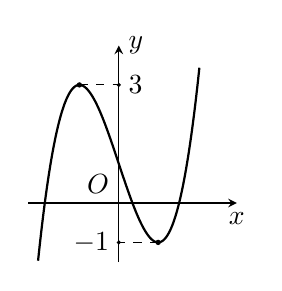
\begin{tikzpicture}[smooth,samples=300,scale=0.5,>=stealth]
			\draw[->] (-2.3,0)--(3,0) node[below]{$x$};
			\draw[->] (0,-1.5)--(0,4) node[right]{$y$};
			\draw (0,0) node[above left]{$O$};
			\draw[thick,domain=-2.05:2.05] plot(\x,{1*((\x)^3)-3*(\x)+1});
			\draw[fill=black] (0,3) circle(1pt) (-1,3) circle(1.5pt) (0,-1) circle(1pt) (1,-1) circle(1.5pt);
			\draw[dashed] (1,-1)--(0,-1)node[left]{$-1$} (-1,3)--(0,3)node[right]{$3$};
		\end{tikzpicture}
	}
	
	\loigiai{
		Ta có $2f(x)-3=0\Leftrightarrow f(x)=\dfrac{3}{2}$.\\
		Từ đồ thị suy ra phương trình có $3$ nghiệm phân biệt.
	}
\end{ex}


\begin{ex}%[2D1B5-3]
	\immini
	{Cho hàm số $f(x)=ax^3 +bx^2 +cx +d$ $(d\ne 0)$ có đồ thị như hình vẽ bên. Số nghiệm của phương trình $3f(x) -1 =0$ bằng
		\haicot
		{$0$}
		{\True $1$}
		{$2$}
		{$3$}
	}
	{\hspace{1cm}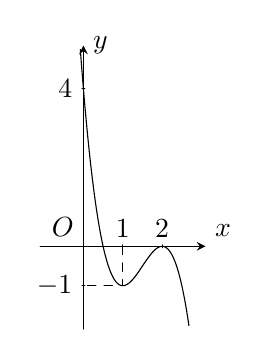
\begin{tikzpicture}[line join=round, line cap=round,>=stealth,scale=0.5]
			\tikzset{label style/.style={font=\footnotesize}}
			\draw[->] (-1.1,0)--(3.1,0) node[above right] {$x$};
			\draw[->] (0,-2.1)--(0,5.1) node[right] {$y$};
			\draw (0,0) node [above left] {$O$};
			\foreach \x in {1,2}
			\draw[thin] (\x,1pt)--(\x,-1pt) node [above] {$\x$};
			\foreach \y in {-1,4}
			\draw[thin] (1pt,\y)--(-1pt,\y) node [left] {$\y$};
			%\draw[dashed,thin](-1,0)--(-1,3)--(0,3);
			\draw[dashed,thin](1,0)--(1,-1)--(0,-1);
			\begin{scope}
				\clip (-1,-2) rectangle (3,5);
				\draw[samples=200,domain=-1:3,smooth,variable=\x] plot (\x,{-2*((\x)^3)+9*((\x)^2)+-12*(\x)+4});
			\end{scope}
	\end{tikzpicture}}
	\loigiai{
		Ta có $3f(x)-1=0 \Leftrightarrow f(x) = \dfrac{1}{3}$.\\
		Khi đó số giao điểm của đồ thị $y=f(x)$ và đường thẳng $y=\dfrac{1}{3}$ chính là số nghiệm của phương trình $3f(x) -1=0$. Dựa vào đồ thị ta có số nghiệm của phương trình là 1.}
\end{ex}

\begin{ex}%[2D1B5-3]
	\immini{Cho hàm số $y = f(x)$ có bảng biến thiên như sau. Số giao điểm của đồ thị hàm số $y = f(x)$ với trục hoành là
		\haicot
		{$ 1$}
		{$ 0$}
		{$ 2  $}
		{\True $ 3 $}}{
		
\begin{tikzpicture}
			\tkzTabInit[lgt=1,espcl=1.8]
			{$x$/0.6, $y’$/0.6, $y$/1.6}
			{$-\infty$,$0$,$1$,$+\infty$}
			\tkzTabLine{ ,-,$0$,+,$0$,-, }
			\tkzTabVar{+/$+\infty$,-/$-1$,+/$3$,-/$-\infty$}
	\end{tikzpicture}}
	\loigiai{
		Dựa vào bảng biến thiên thì đồ thị hàm số $y = f(x)$ và trục hoành có $3$ điểm chung.	
	}
\end{ex}

\begin{ex}%[2D1B5-3]
	\immini{Cho hàm số $y=f(x)$ liên tục trên $(-\infty;+\infty)$ và có bảng biến thiên như hình bên. Số nghiệm thực của phương trình $2\big|f(x)\big|=7$ bằng
		\choice
		{$3$}
		{\True $2$}
		{$4$}
		{$2$}	
		
		
	}{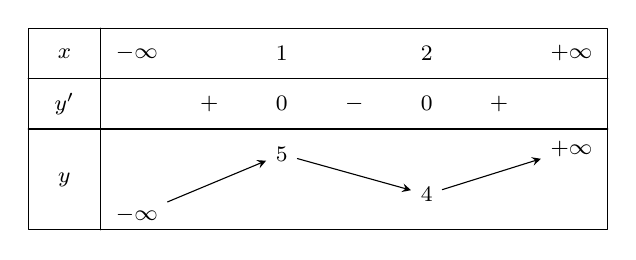
\begin{tikzpicture}[>=stealth,line join=round,line cap=round,font=\footnotesize,scale=.8]
			\begin{scope}[xscale=1.15,yscale=0.8]
				\begin{scope}[shift={(-0.5,0.5)}]
					\def\a{8}
					\def\b{4}
					\draw (0,0)rectangle +(\a,-\b)
					(1,0)--+(-90:\b)
					(0,-1)--+(0:\a)
					(0,-2)--+(0:\a)
					;
				\end{scope}
				\draw
				(0,0)node{$x$}++(0:1)node{$-\infty$}++(0:2)node{$1$}++(0:2)node{$2$}
				++(0:2)node{$+\infty$}
				(0,-1)node{$y'$}	++(0:2)node{$+$}++(0:1)node{$0$}++(0:1)node{$-$}++(0:1)node{$0$}++(0:1)node{$+$}
				(0,-2.5)node{$y$}
				(1,-3.2) node (A)  {$-\infty$} 
				(3,-2)node (B) {$5$} 
				(5,-2.8) node (C){$4$} 
				(7,-1.9)node (D){$+\infty$} 
				;
				\draw[->] (A)--(B);
				\draw[->] (B)--(C);
				\draw[->] (C)--(D);
			\end{scope}	
	\end{tikzpicture}}
	
	\loigiai{
		
	}
\end{ex}

\begin{ex}%[2D1K5-3]
	\immini{Cho hàm số $y=f(x)$ liên tục trên $\mathbb{R}\setminus\{0\}$ và có bảng biến thiên như hình bên. Hỏi phương trình $3|f(x)|-10=0$ có bao nhiêu nghiệm?
		\choice
		{$2$ nghiệm}
		{$4$ nghiệm}
		{\True $3$ nghiệm}
		{$1$ nghiệm}
	}{
		
\begin{tikzpicture}
			\tikzset{double style/.append style = {draw=\tkzTabDefaultWritingColor,double=\tkzTabDefaultBackgroundColor,double distance=2pt}}
			\tkzTabInit[nocadre=false,lgt=1.2,espcl=1.7,deltacl=0.6]
			{$x$ /.6,$f'(x)$ /.6,$f(x)$ /1.7}{$-\infty$,$0$,$1$,$+\infty$}
			\tkzTabLine{,-,d,-,0,+,}
			\tkzTabVar{+/$2$,-D+/$-\infty$/+$\infty$,-/$3$,+/$+\infty$}
	\end{tikzpicture}}
	\loigiai
	{
		Từ bảng biến thiên đề bài, ta có bảng biến thiên của hàm số $y=|f(x)|$ như sau
		\begin{center}
			
\begin{tikzpicture}
				\tkzTabInit[nocadre=false,lgt=1.3,espcl=2.5,deltacl=0.6]
				{$x$ /.6,$f'(x)$ /.6,$|f(x)|$ /2}{$-\infty$,,$0$,$1$,$+\infty$}
				\tkzTabLine{,,-,,d,-,0,+,}
				\tkzTabVar{+/$2$,-/$0$,+D+/$+\infty$/+$\infty$,-/$3$,+/$+\infty$}
			\end{tikzpicture}
		\end{center}
		Ta có $3|f(x)|-10=0\Leftrightarrow |f(x)|=\dfrac{10}{3}.\qquad(1)$\\
		Số nghiệm của phương trình (1) bằng số giao điểm của đồ thị $y=|f(x)|$ và đường thẳng $y=3$.\\
		Dựa vào bảng biến thiên trên, suy ra phương trình (1) có $3$ nghiệm. 
	}
\end{ex}

\begin{ex}%[2D1K5-3]
	\immini{Cho hàm số $y = f(x)$ xác định và liên tục trên $\mathbb{R}$, có bảng biến thiên như sau. Số nghiệm của phương trình $2[f(x)]^2- 3 f(x)+ 1 = 0$ là
		\haicot
		{$2$}
		{\True $3$}
		{$6$}
		{$0$}}
	{
\begin{tikzpicture}[scale=0.8]
			\tkzTabInit[espcl=2.3,lgt=1.2,deltacl=0.6]
			{$x$/0.6,$y'$/0.6,$y$/2}
			{$-\infty$,$-1$,$1$,$+\infty$}
			\tkzTabLine{,+,0,-,0,+,}
			\tkzTabVar{-/$1$,+/$3$,-/$\dfrac{1}{3}$,+/$1$}
	\end{tikzpicture}}
	\loigiai{
		Ta có $ 2[f(x)]^2- 3 f(x)+ 1 = 0\Leftrightarrow \left[\begin{array}{l}{f(x)= 1}\\{f(x)= \dfrac{1}{2}.}\end{array}\right.$\\
		Phương trình $f(x)= 1$ có duy nhất nghiệm $ x_0 $.\\
		Phương trình $f(x)= \dfrac{1}{2}$ có $2$ nghiệm phân biệt khác $x_{0}$.  Vậy phương trình có ba nghiệm.
	}
\end{ex}

\begin{ex}
	\immini{Cho hàm số $f(x)$ có bảng biến thiên như hình bên. Tìm tất cả các giá trị thực của tham số $m$ để phương trình $f(x)=m+1$ có ba nghiệm thực phân biệt.
		\choice
		{$-3\le m \le 3$}
		{$-2\le m \le 4$}
		{$-2<m<4$}
		{\True $-3<m<3$}
	}{
		
\begin{tikzpicture}
			\tkzTabInit[nocadre=false,lgt=1,espcl=1.9,deltacl=0.6]
			{$x$ /0.6, $y'$ /0.6, $y$ /1.6}
			{$-\infty$,$-1$,$3$,$+\infty$}
			\tkzTabLine{,+,$0$,-,$0$,+,}
			\tkzTabVar{-/$-\infty$,+/$4$,-/$-2$,+/$+\infty$}
	\end{tikzpicture}}
	\loigiai{
		Dựa vào bảng biến thiên phương trình $f(x)=m+1$ có ba nghiệm thực phân biệt khi
		\begin{center}
			$-2<m+1<4 \Leftrightarrow -3<m<3$.
		\end{center}
	}
\end{ex}

\begin{ex}
	\immini{Cho hàm số $y=f(x)$ có bảng biến thiên như hình bên. Phương trình $f(4x-x^2)-2=0$ có bao nhiêu nghiệm thực?
		\choice 
		{$2$}
		{$6$}
		{$0$}
		{\True $4$}
	}{
		
\begin{tikzpicture}
			\tkzTabInit[nocadre=false,lgt=1.2,espcl=2.2,deltacl=0.6]
			{$x$ /0.6,$y’$ /0.6,$y$ /1.6}
			{$-\infty$ ,$0$ , $4$, $+\infty$}
			\tkzTabLine{,-,0,+,0,-}
			\tkzTabVar{+/ $+\infty $ / , -/ $-1$ /,+/ $3$/ , -/ $-\infty$ /}  
	\end{tikzpicture} }
	\loigiai{ 
		Đặt $t=4x-x^2$. Khi đó $t=-(x-2)^2+4 \leq 4$.\\
		Từ mỗi giá trị $t<4$ ta tìm được hai giá trị $x$. Với $t=4$ ta tìm được $x=2$.\\
		Từ bảng biến thiên, ta thấy phương trình $f(t)=2 \Leftrightarrow \left [ \begin{aligned} &t=\alpha \in (-\infty;0)\\ 
			&t=\beta \in (0;4)  \\
			&t=\gamma \in  (4;+\infty)  \end{aligned} \right.$\\
		Vậy phương trình $f(4x-x^2)-2=0$ có $4$ nghiệm. 
	}   
\end{ex}

\Closesolutionfile{ans}

